% 平面波
% 平面波|简谐波|简谐振子|角频率|波速|波长|周期

\pentry{矢量内积\upref{Dot}, 简谐振子\upref{SHO}}

通常我们说 “波” 时, 它几乎可以是任意形状的, 例如一个波包\upref{WvPck}. 但我们先来讨论一种最简单的波动, 叫做\textbf{简谐波(sinusoidal wave)}, 在任意时刻, 它在传播方向的波形是一个正弦函数. 简谐波也叫\textbf{平面波(plane wave)}, 本书对这两个词不加区分. 叫平面波是因为三维平面波的等相位面都是平面, 但其他维度习惯上也可以使用这个词, 这在量子力学中较常见\footnote{见几乎任意一本常见量子力学入门教材}.

\subsection{一维情况}
我们先来看一个一维的平面波, 一个常用的例子是一根无限长的弦, 静止的时候弦与 $x$ 轴重合, 在任何时刻 $t$, 弦的波函数(即形状)可以用 $y(x, t)$ 来描述. 若
\begin{equation}\label{PWave_eq1}
y(x, t) = A\cos(k x - \omega t + \varphi_0)
\end{equation}
则我们把这个波函数称为\textbf{平面波}, 如\autoref{PWave_fig1} 所示\footnote{需要注意的是,图中的横轴是位置 $x$ 而不是时间 $t$, 要避免将质点振动的位移—时间图与该图混淆.}.

\begin{figure}[ht]
\centering
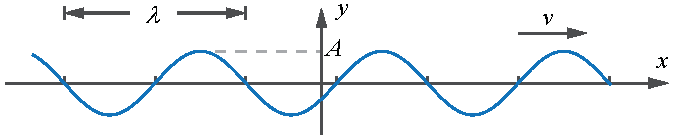
\includegraphics[width=12cm]{./figures/PWave_1.pdf}
\caption{平面波} \label{PWave_fig1}
\end{figure}

我们定义图中的 $A$ 为振幅, 定义一个空间周期为\textbf{波长(wave length)}, 记为 $\lambda$. 与波长一一对应的一个量是\autoref{PWave_eq1} 中的 $k$, 称为\textbf{波数(wave number)}. 波长与波数的关系可以类比简谐振子\upref{SHO} 的角频率 $\omega$ 与时间周期 $T$ 的关系, 即
\begin{equation}
k = \frac{2\pi}{\lambda}
\end{equation}

我们再来看波函数随时间的变化, 如果在弦的某个位置做一个标记并观察其运动, 则\autoref{PWave_eq1} 中 $x$ 可视为常数, 我们立即得到一个简谐振动, 角频率为 $\omega$, 初相位为\footnote{由于余弦函数是偶函数, 我们不妨将 $\cos$ 的自变量取相反数使 $\omega t$ 的符号为正.} $-kx - \varphi_0$.

我们在观察平面波的时候, 通常会想象它在移动(虽然弦上每个点的 $x$ 坐标并不改变), 我们把这种移动的速度叫做\textbf{波速(wave velocity)} $v$. 把\autoref{PWave_eq1} 稍作整理得
\begin{equation}
y(x, t) = A\cos \qty[k \qty(x - \frac{\omega}{k} t) + \varphi_0]
\end{equation}
由于函数 $f(x - x_0)$ 可以看做 $f(x)$ 向 $x$ 轴正方向平移 $x_0$ 得到的函数, 上式也可以看做 $t = 0$ 时刻的波函数向 $x$ 轴正方向平移 $\omega t/k$ 得到的波函数. 将平移距离除以 $t$ 就得到了单位时间移动的距离, 即波速
\begin{equation}
v = \frac{\omega}{k}
\end{equation}
如果将 $\omega = 2\pi/T$ 和 $k = 2\pi/\lambda$ 代入上式, 得到波速的另一个表达式
\begin{equation}
v = \frac{\lambda}{T}
\end{equation}
这里的 $T$ 是振动周期. 也可以令振动频率 $f = 1/T$, 则上式又变为
\begin{equation}
v = \lambda f
\end{equation}

\subsection{横波与纵波}
以上我们看到的波函数表示\textbf{横波}, 即质点振动的方向与波的传播方向垂直. 与横波相对的另一类波叫做\textbf{纵波}, 即质点振动方向与波的传播方向相同. 纵波的波函数与横波相同, 只是函数值的意义由垂直方向的位移改为了平行方向的位移(不妨记为 $\xi$)
\begin{equation}
\xi = A \cos(k x - \omega t + \varphi_0)
\end{equation}
广义来说, 振幅可以是一个任意方向的矢量 $\bvec A$, 它可以既不平行也不垂直于传播方向.

\subsection{二维和三维的平面波}

\begin{figure}[ht]
\centering
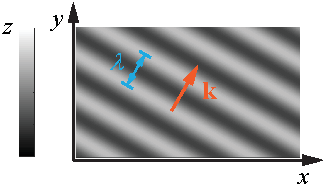
\includegraphics[width=5.7cm]{./figures/PWave_2.pdf}
\caption{二维平面波} \label{PWave_fig2}
\end{figure}

如\autoref{PWave_fig2}, 我们可以用函数 $z(x,y,t)$ 表示一个二维的平面波(横波). 波长的定义与一维情况相同, 在 $k = 2\pi/\lambda$ 的基础上, 我们定义\textbf{波矢} $\bvec k$ 的方向为波速的方向.
观察图中的波可以发现, 沿波矢方向移动 $l$, 相位变化为 $kl$, 沿垂直波矢方向移动 $l$, 相位不改变, 沿任意其他方向移动 $l$, 相位变化为 $kl\cos\theta$, 其中 $\theta$ 是移动方向与 $\bvec k$ 方向的夹角. 于是我们可以用内积来表示相位随空间的变化
\begin{equation}
\Delta\varphi = \bvec k \vdot \Delta\bvec r = k_x \Delta x + k_y \Delta y
\end{equation}
于是我们可以写出波函数为
\begin{equation}\label{PWave_eq8}
z = A \cos(\bvec k \vdot \bvec r - \omega t + \varphi_0)
\end{equation}
要表示纵波, 同样把 $z$ 换位 $\xi$ 即可.

类似地, 三维空间中的平面波可表示为
\begin{equation}
\bvec s = \bvec A \cos(\bvec k \vdot \bvec r - \omega t + \varphi_0)
\end{equation}
其中 $\bvec k$ 和 $\bvec r$ 是三维矢量. 注意这里的 $\bvec r$ 表示介质静止时某质点的位矢. 如果波函数表示横波, 矢量振幅 $\bvec A$ 必须垂直于波矢 $\bvec k$, 其方向叫做\textbf{极化方向}. 如果波函数表示纵波, $\bvec A$ 必须与 $\bvec k$ 同向.

\subsection{波函数的复数表示}
\pentry{振动的指数形式\upref{VbExp}}

用复数表示波函数,往往可以化简书写和计算. 类比\autoref{VbExp_eq3}~\upref{VbExp}, 我们可以把平面波表示为指数形式\footnote{现在我们知道为什么振动的指数形式中 $\omega t$ 要带一个负号了, 这样就可以让波动的指数形式中 $\bvec k\vdot \bvec r$ 项为正.}
\begin{equation}
\tilde {\bvec s} = \bvec A \E^{\I( \bvec k \vdot \bvec r - \omega t + \varphi_0)}
\end{equation}
注意只有实部表示质点的位移, 虚部无物理意义.

